\documentclass[11pt]{article}
\usepackage{amsmath, amssymb, physics, mathtools, bm}
\usepackage{tikz}
\usetikzlibrary{decorations.markings, decorations.pathmorphing, arrows.meta}
\usepackage[margin=2.3cm]{geometry}
\usepackage{siunitx, booktabs, hyperref}
\usepackage{braket}

\newcommand{\D}{\mathrm{D}}
\newcommand{\de}{\mathrm{d}}
\newcommand{\pd}[2]{\frac{\partial #1}{\partial #2}}
\newcommand{\pdd}[2]{\frac{\partial^{2} #1}{\partial #2^{2}}}
\newcommand{\Lap}{\nabla^{2}}
\newcommand{\lambdabar}{\ensuremath{\mathchar'26\mkern-9mu\lambda}}

\title{B4 --- Nuclear and Particle Physics: Model Solutions, Trinity 2023}
\author{}
\date{}

\begin{document}
\maketitle

\section*{Question 1 --- Isospin, hadronic scattering, antiproton threshold}

\textbf{Problem statement.} The question asks for the origin of isospin and the conditions
under which it is conserved or violated in the strong, weak, and electromagnetic
interactions; the total isospin of $p\pi^{\pm}$ systems; an interpretation of the symmetric
forward/backward peaks in $\sim 1$\,GeV $pn$ elastic scattering using effective pion
exchange diagrams (with colour conserved); a derivation of the modified antiproton
threshold in nuclei due to the internal Fermi momentum $q$; the identification of the
mediators in $p\bar p \to \pi^+\pi^-$; the connection between the gluon's self-coupling and
confinement/asymptotic freedom; and a check of the conservation laws in
$\pi^- p \to \pi^-\pi^0\pi^+ n$.

\subsection*{(a) Origin and status of isospin}

Isospin originated from Heisenberg's observation that the proton and neutron have nearly
equal masses ($m_n - m_p \simeq 1.3\,\mathrm{MeV}$, an effect of order $10^{-3}$ relative
to the nucleon mass) and that the strong nuclear force between $pp$, $pn$, and $nn$ pairs is,
to a good approximation, charge independent. He proposed regarding $p$ and $n$ as two
states of a single object, the nucleon, transforming as an $\mathrm{SU(2)}$ doublet
\begin{equation}
N=\begin{pmatrix}p\\ n\end{pmatrix}, \qquad I=\tfrac{1}{2},\;\; I_3=+\tfrac{1}{2}\text{ for }p,\;\; I_3=-\tfrac{1}{2}\text{ for }n.
\label{eq:nucleon-doublet}
\end{equation}
At the quark level isospin is the approximate $\mathrm{SU(2)}$ symmetry that exchanges
the $u$ and $d$ quarks; it would be \emph{exact} if $m_u=m_d$ and the quark electric
charges were equal.

Isospin is therefore an \emph{approximate} global symmetry, not an exact one. The strong
interaction is flavour-blind --- the gluon coupling is the same to $u$ and $d$ quarks --- so
the strong force conserves isospin to a level set only by the small $u$--$d$ mass difference
$m_d-m_u\sim 3\,\mathrm{MeV}$, much smaller than typical hadronic scales of
$\Lambda_\mathrm{QCD}\sim 200\,\mathrm{MeV}$. The electromagnetic interaction violates
isospin because the photon couples differently to $u$ ($Q=+2/3$) and $d$ ($Q=-1/3$);
$I_3$ is conserved (charge is conserved and the electromagnetic current carries no net
isospin change beyond $I_3$) but the total $I$ is not. The weak interaction violates isospin
maximally: the charged $W$ couples only to left-handed fermions and connects different
generations, and the up- and down-type quark masses differ greatly, so neither $I$ nor (in
flavour-changing processes) $I_3$ is conserved.

\subsection*{(b) Total isospin of $p\pi^{\pm}$}

The proton has $I=\tfrac{1}{2}$ and the pion triplet has $I=1$. Combining a doublet with
a triplet using $\mathrm{SU(2)}$ addition gives
\begin{equation}
\tfrac12 \otimes 1 = \tfrac12 \oplus \tfrac32,
\label{eq:isospin-decomp}
\end{equation}
so a $p+\pi$ system has total isospin $I=\tfrac{1}{2}$ or $I=\tfrac{3}{2}$.

(i) For $p\pi^+$, $I_3 = +\tfrac12 + 1 = +\tfrac32$. Only $I=\tfrac32$ contains the
$I_3=+\tfrac32$ projection, so this is a pure $I=\tfrac{3}{2}$ state:
\begin{equation}
\boxed{\,\ket{p\pi^+}=\ket{\tfrac32,+\tfrac32}.\,}
\end{equation}

(ii) For $p\pi^-$, $I_3 = +\tfrac12 - 1 = -\tfrac12$, which is contained in both
$I=\tfrac32$ and $I=\tfrac12$. Using Clebsch--Gordan coefficients,
\begin{equation}
\boxed{\,\ket{p\pi^-}=\sqrt{\tfrac13}\,\ket{\tfrac32,-\tfrac12}-\sqrt{\tfrac23}\,\ket{\tfrac12,-\tfrac12}.\,}
\end{equation}
The two pure isospin amplitudes interfere in the cross section, which is why the famous
ratio $\sigma(\pi^+ p)/\sigma(\pi^- p)=9$ at the $\Delta(1232)$ resonance probes a pure
$I=\tfrac32$ intermediate state.

\subsection*{(c) Symmetric forward/backward peaks in $pn$ elastic scattering}

The forward peak ($\cos\theta\to+1$) is the usual diffractive elastic peak, where the
incoming proton continues forward after a small-angle scatter. The backward peak
($\cos\theta\to-1$) cannot be diffractive: it represents events in which the
\emph{identity} of the outgoing forward particle has changed --- the original proton has
become a neutron, and what comes out forward is the original target neutron now turned
into a proton. This is charge exchange: a $\pi^+$ has been transferred from projectile to
target.

A backward peak in elastic scattering between identical particles is forbidden by Bose
statistics for bosons and by Fermi statistics for identical fermions, but here $p$ and $n$
are distinguishable: the only way the angular distribution can be symmetric is if the
outgoing proton in the c.m.~frame is, with equal weight, either the original projectile
(forward) or the original target after $\pi^+$ exchange (backward). Effective one-pion
exchange is the long-range part of the strong nucleon--nucleon interaction (Yukawa) and
captures both topologies.

\emph{Forward peak --- $\pi^0$ exchange (no charge transfer).} The incoming proton emits
a $\pi^0=(u\bar u-d\bar d)/\sqrt2$ which is absorbed by the neutron; both nucleons retain
their identity. At quark level a $u\bar u$ pair is exchanged: the proton momentarily
splits into $(uud)\to(ud)+u\bar u/\sqrt2$, the $u\bar u$ propagates as a colour-singlet
$\pi^0$, and is absorbed by the neutron $(udd)$. Each ``side'' of the diagram is a
colour singlet $q\bar q$ pair; equivalently, the exchanged pion is $1/\sqrt3\,(R\bar R+G\bar
G+B\bar B)$, so colour is exchanged but the net colour transferred to either nucleon is
zero.

\emph{Backward peak --- $\pi^+$ exchange (charge exchange).} The incoming proton $(uud)$
emits a $\pi^+=u\bar d$ and becomes a neutron $(udd)$; the target neutron $(udd)$ absorbs
the $\pi^+$ and becomes a proton $(uud)$. In the c.m.~frame the outgoing proton therefore
emerges in the direction the incoming neutron was originally moving, i.e.~backward
relative to the incoming proton, hence the backward peak.

\begin{center}
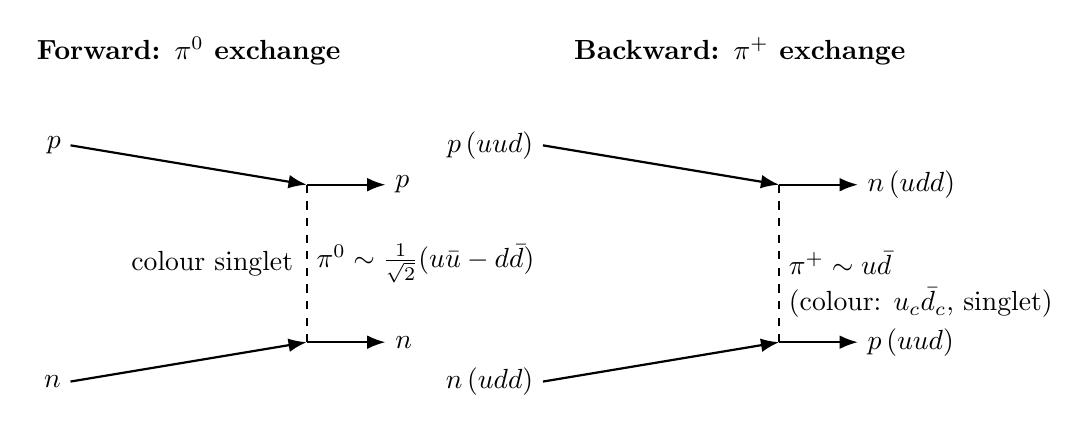
\begin{tikzpicture}[scale=1.0,>=Latex]
% forward (pi^0)
\node at (-3.5,3.2) {\textbf{Forward: $\pi^0$ exchange}};
\draw[->,thick] (-5,2)--(-2,1.5);  \node[left] at (-5,2) {$p$};
\draw[->,thick] (-2,1.5)--(-1,1.5); \node[right] at (-1,1.5) {$p$};
\draw[->,thick] (-5,-1)--(-2,-0.5); \node[left] at (-5,-1) {$n$};
\draw[->,thick] (-2,-0.5)--(-1,-0.5); \node[right] at (-1,-0.5) {$n$};
\draw[dashed,thick] (-2,1.5)--(-2,-0.5);
\node[right] at (-2,0.5) {$\pi^0\sim\tfrac{1}{\sqrt2}(u\bar u-d\bar d)$};
\node[left] at (-2.05,0.5) {colour singlet};
% backward (pi^+)
\node at (3.5,3.2) {\textbf{Backward: $\pi^+$ exchange}};
\draw[->,thick] (1,2)--(4,1.5);  \node[left] at (1,2) {$p\,(uud)$};
\draw[->,thick] (4,1.5)--(5,1.5); \node[right] at (5,1.5) {$n\,(udd)$};
\draw[->,thick] (1,-1)--(4,-0.5); \node[left] at (1,-1) {$n\,(udd)$};
\draw[->,thick] (4,-0.5)--(5,-0.5); \node[right] at (5,-0.5) {$p\,(uud)$};
\draw[dashed,thick] (4,1.5)--(4,-0.5);
\node[right] at (4,0.5) {$\pi^+\sim u\bar d$};
\node[right] at (4,0.0) {(colour: $u_c\bar d_c$, singlet)};
\end{tikzpicture}
\end{center}

In each diagram the exchanged $q\bar q$ pair carries quark colour $c$ and antiquark colour
$\bar c$ summed coherently to form a colour-singlet meson, so the net colour transferred
between the nucleons is zero --- colour confinement is respected.

\subsection*{(d) Antiproton-production threshold with internal Fermi momentum}

For antiproton production on a free, stationary proton target, $p+p\to p+p+p+\bar p$, the
minimum-energy configuration in the lab is when all four final-state nucleons emerge at
rest in the c.m.~frame. Calling $E_\mathrm{min}$ the minimum incident energy and using
the invariant
\begin{equation}
s=(E_\mathrm{min}+m_p c^2)^2-(p_\mathrm{min} c)^2 = (4 m_p c^2)^2,
\label{eq:s-free}
\end{equation}
together with $E_\mathrm{min}^2 - (p_\mathrm{min} c)^2 = (m_p c^2)^2$, one obtains
$E_\mathrm{min}=7\,m_p c^2$, of which $6\,m_p c^2$ is kinetic, the well-known result.

When the target nucleon belongs to a nucleus and possesses Fermi momentum $\mathbf q$,
the most favourable kinematic configuration is when $\mathbf q$ points \emph{antiparallel}
to the incoming beam, so that the projectile and target approach head-on with the maximum
relative momentum. Writing the target four-momentum as $(E_T, -q\hat z)$ with
$E_T=\sqrt{q^2c^2+m_p^2 c^4}\simeq m_p c^2 + q^2/(2m_p)$, the invariant
\begin{equation}
s'=(E'_\mathrm{min}+E_T)^2-(p'_\mathrm{min}c-qc)^2 = (4 m_p c^2)^2
\label{eq:s-fermi}
\end{equation}
must again equal $(4m_p c^2)^2$. Expanding,
\begin{equation}
E'^2_\mathrm{min}-p'^2_\mathrm{min}c^2 + 2E'_\mathrm{min}E_T + 2 p'_\mathrm{min}c\,qc + E_T^2 - q^2c^2 = 16 m_p^2 c^4.
\label{eq:s-expand}
\end{equation}
The first term is $m_p^2 c^4$ and the last two combine to $m_p^2 c^4$, giving
$2 E'_\mathrm{min}E_T+2p'_\mathrm{min}qc^2=14 m_p^2 c^4$. To leading order in $q$ we
may set $E_T\simeq m_p c^2$ and $p'_\mathrm{min}c\simeq E'_\mathrm{min}$ (since the
threshold beam is highly relativistic, $E_\mathrm{min}\gg m_p c^2$), so
\begin{equation}
2 E'_\mathrm{min} m_p c^2 + 2 E'_\mathrm{min} q c = 14 m_p^2 c^4 \;\Longrightarrow\; E'_\mathrm{min} = \frac{7 m_p^2 c^4}{m_p c^2 + qc}=\frac{E_\mathrm{min}}{1+q/(m_p c)}.
\label{eq:Eprime}
\end{equation}
Expanding to first order in $q/(m_p c)$,
\begin{equation}
\boxed{\;E'_\mathrm{min}\simeq E_\mathrm{min}\left(1-\frac{q}{m_p c}\right).\;}
\label{eq:final-threshold}
\end{equation}
Numerically, the antiproton was discovered with a $\sim 6.2$\,GeV proton beam on a copper
target instead of the free-target threshold $E_\mathrm{kin}=6 m_p c^2\simeq 5.6$\,GeV
(total $E_\mathrm{min}\simeq 6.6$\,GeV), i.e.~a reduction of about
$\Delta E_\mathrm{min}/E_\mathrm{min}\sim 0.06$. Equation~\eqref{eq:final-threshold}
then yields
\begin{equation}
q\sim 0.06\, m_p c \simeq 60\,\mathrm{MeV}/c,
\end{equation}
in good agreement with the standard estimate of the nuclear Fermi momentum
$p_F\simeq 250\,\mathrm{MeV}/c$ averaged over the Fermi sphere (the relevant quantity is
the mean of $|\mathbf q\cdot\hat z|$, not $p_F$). One quotes
$\boxed{\,q\sim 0.05\text{--}0.1\,m_p c \approx 50\text{--}100\,\mathrm{MeV}/c.\,}$

\subsection*{(e) $p\bar p\to\pi^+\pi^-$ as effective hadron exchange}

In the quark picture the proton is $(uud)$ and the antiproton is $(\bar u\bar u\bar d)$, while
$\pi^+=u\bar d$ and $\pi^-=\bar u d$. Two annihilation/exchange topologies are possible.

\emph{Doubly charged exchange ($\Delta^{++}$-like).} Two $u$ quarks of the proton combine
with two $\bar u$ quarks of the antiproton through an exchanged object that carries the
quark content $uu\bar u\bar u$. Splitting it as $(uud)+(\bar u\bar d)\to(u\bar d)$ on the
proton side and $(\bar u\bar u\bar d)+(ud)\to(\bar u d)$ on the antiproton side, the
$t$-channel propagator is a state with quark content $u u \bar d \bar d$ minus the spectators
--- effectively a doubly-charged hadron $\Delta^{++}=uuu$ exchange would balance charge if
viewed as a $u u$-baryon line. More cleanly: the $u$-quark from the proton joins the $\bar
d$ produced from the sea to form the outgoing $\pi^+$, and the $\bar u$ from the antiproton
joins the $d$ from the sea to form the $\pi^-$. The exchanged quanta in $t$-channel are
the diquark--antidiquark pair which has the quantum numbers of a doubly charged
$\Delta^{++}=uuu$ baryon (an $I=\tfrac32$, $Q=+2$ resonance).

\emph{Neutral exchange ($\rho^0$- or $\omega$-like).} The other topology is annihilation in
the $s$-channel: $u\bar u$ (or $d\bar d$) annihilates to a colour-singlet $q\bar q$
intermediary which subsequently fragments to $\pi^+\pi^-$. The relevant intermediaries are
the neutral vector mesons that couple to two pions: the $\rho^0(770)$ ($I=1$, $J^P=1^-$)
and the $\omega(782)$ ($I=0$, $J^P=1^-$). Of these, $\rho^0\to\pi^+\pi^-$ has branching
ratio $\sim 100\%$, while $\omega\to\pi^+\pi^-$ is $G$-parity suppressed and only $\sim 1.5\%$.

\begin{center}
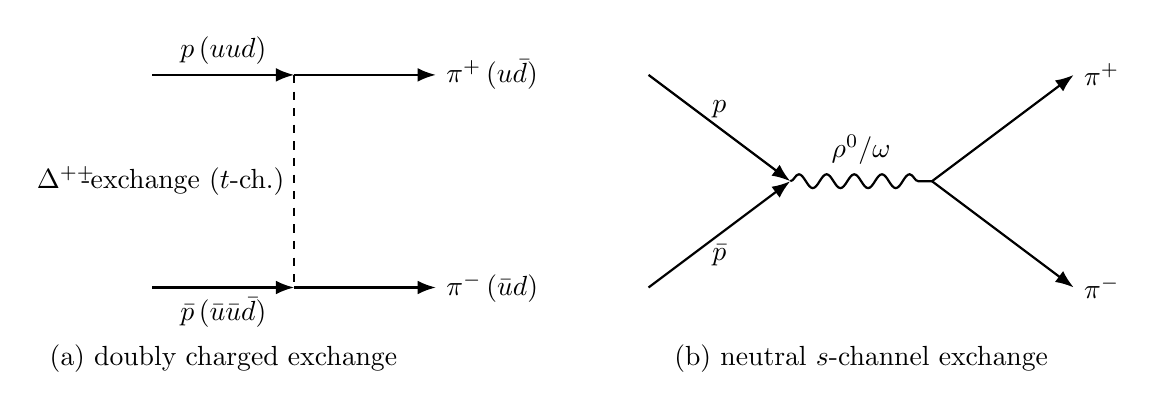
\begin{tikzpicture}[scale=0.9,>=Latex]
\draw[->,thick](-4,1.5)--(-2,1.5)node[midway,above]{$p\,(uud)$};
\draw[->,thick](-4,-1.5)--(-2,-1.5)node[midway,below]{$\bar p\,(\bar u\bar u\bar d)$};
\draw[->,thick](-2,1.5)--(0,1.5)node[right]{$\pi^+\,(u\bar d)$};
\draw[->,thick](-2,-1.5)--(0,-1.5)node[right]{$\pi^-\,(\bar u d)$};
\draw[dashed,thick](-2,1.5)--(-2,-1.5);
\node[left] at (-2,0) {$\Delta^{++}\!\!\!$-exchange ($t$-ch.)};
\node at (-3,-2.5) {(a) doubly charged exchange};
% s-channel
\draw[->,thick](3,1.5)--(5,0)node[midway,above]{$p$};
\draw[->,thick](3,-1.5)--(5,0)node[midway,below]{$\bar p$};
\draw[decorate,decoration={snake},thick](5,0)--(7,0);
\node[above] at (6,0.1) {$\rho^0/\omega$};
\draw[->,thick](7,0)--(9,1.5)node[right]{$\pi^+$};
\draw[->,thick](7,0)--(9,-1.5)node[right]{$\pi^-$};
\node at (6,-2.5) {(b) neutral $s$-channel exchange};
\end{tikzpicture}
\end{center}

\subsection*{(f) Mediator self-coupling, confinement and asymptotic freedom}

The crucial difference is that the photon, the mediator of QED, is electrically neutral and
therefore does not couple to itself, while the gluon, the mediator of QCD, carries colour
charge (it transforms in the $\mathrm{SU(3)}$ adjoint, $3\otimes\bar 3 = 1\oplus 8$, eight
coloured gluons). Gluon self-coupling produces three- and four-gluon vertices.

The non-Abelian self-coupling has two consequences. First, the chromoelectric flux lines
between a quark and an antiquark are squeezed by gluon--gluon attraction into a tube of
roughly constant energy per unit length $\sigma\sim 1$\,GeV/fm, so separating the quarks
costs linearly growing energy --- this is \emph{confinement}. Second, the loop correction
to the gluon propagator includes both fermion loops (which screen, as in QED) and gluonic
loops (which anti-screen, with no QED analogue). The anti-screening dominates for
$N_c=3$, $N_f\le 16$, giving a negative QCD beta function and the running coupling
$\alpha_s(\mu)\to 0$ as $\mu\to\infty$ --- this is \emph{asymptotic freedom}.

\subsection*{(g) Allowedness of $\pi^- p\to\pi^-\pi^0\pi^+ n$}

We check the conserved quantum numbers in turn. Charge: LHS $-1+1=0$, RHS $-1+0+1+0=0$
\checkmark. Baryon number: LHS $0+1=1$, RHS $0+0+0+1=1$ \checkmark. Lepton number is
trivially conserved (none on either side). Strangeness, charm, etc.~are all zero on both
sides. The energy budget is also trivially fine for an above-threshold reaction (the
$\pi^- p$ c.m.~energy needed is $m_n+3m_\pi\simeq 940+420\simeq 1360$\,MeV, well within
beam reach). Isospin is approximately conserved by the strong interaction; both sides
contain accessible $I=\tfrac12$ and $I=\tfrac32$ components, so this is not a barrier.

The reaction is therefore \emph{allowed} as a strong-interaction process. A representative
dominant Feynman diagram is single-pion exchange between the projectile and target, with
the projectile pion ``shaking off'' an extra $\pi^+\pi^-$ pair (a $\rho^0$ or virtual $\sigma$
intermediate), and the target proton converting to a neutron by emitting a $\pi^+$ which
recombines with the radiated $q\bar q$ pair --- equivalent to the dominant
``pion bremsstrahlung'' topology.

\begin{center}
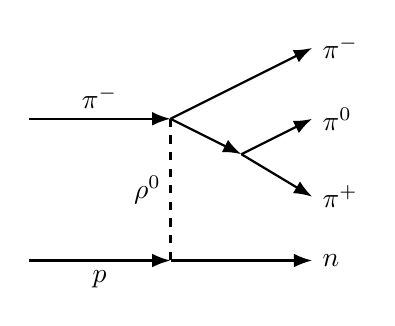
\begin{tikzpicture}[scale=0.9,>=Latex]
\draw[->,thick] (-4,1.5)--(-2,1.5) node[midway,above]{$\pi^-$};
\draw[->,thick] (-2,1.5)--(0,2.5) node[right]{$\pi^-$};
\draw[->,thick] (-2,1.5)--(-1,1) ;
\draw[->,thick] (-1,1)--(0,1.5) node[right]{$\pi^0$};
\draw[->,thick] (-1,1)--(0,0.4) node[right]{$\pi^+$};
\draw[dashed,thick] (-2,1.5)--(-2,-0.5);
\node[left] at (-2,0.5) {$\rho^0$};
\draw[->,thick] (-4,-0.5)--(-2,-0.5) node[midway,below]{$p$};
\draw[->,thick] (-2,-0.5)--(0,-0.5) node[right]{$n$};
\end{tikzpicture}
\end{center}
This is a strong process at tree level, with all exchanges colour-singlet hadronic and all
vertices flavour-conserving. Hence the reaction is allowed and proceeds via the strong
interaction.

\section*{Question 2 --- $W$ production, Breit--Wigner, and the $e^+e^-\to$\,hadrons spectrum}

\textbf{Problem statement.} The question requires three leading-order Feynman diagrams for
$W$-boson production at an $e^+e^-$ collider, the $W$ decay modes and how each is detected
in a hermetic detector, the relativistic Breit--Wigner cross section and its non-relativistic
limit, and the identification and physical interpretation of resonances $a$--$f$ in the
$e^+e^-\to\mathrm{hadrons}$ cross section.

\subsection*{(a) Leading-order $W$ production in $e^+e^-$}

Three distinct exchange topologies produce $W$ bosons in $e^+e^-$ annihilation.

\emph{(i) $s$-channel single-$W$ via $W$--$\gamma$ or $W$--$Z$ fusion vanishes at LO};
the lowest-order single-$W$ production is via radiative return / $Wev$ ``$t$-channel''
single-$W$:
\begin{equation}
e^+e^-\to W^\pm \ell^\mp \nu_\ell \quad (t\text{-channel }W \text{ from one of the leptons}),
\end{equation}
where one of the incoming leptons radiates a $W$ off its line, with a neutrino in the
final state.

\emph{(ii) $s$-channel $\gamma^*/Z^*\to W^+ W^-$ pair production:}
\begin{equation}
e^+e^-\to \gamma^*/Z^*\to W^+ W^-,
\end{equation}
the dominant LEP-2 process for $\sqrt s>2 M_W$, using the triple-gauge $\gamma WW$ and
$ZWW$ vertices.

\emph{(iii) $t$-channel neutrino exchange:}
\begin{equation}
e^+e^-\to W^+W^- \quad \text{via }t\text{-channel } \nu_e,
\end{equation}
where the electron emits a $W^-$ becoming a $\nu_e$, which then absorbs the positron with
emission of a $W^+$.

\begin{center}
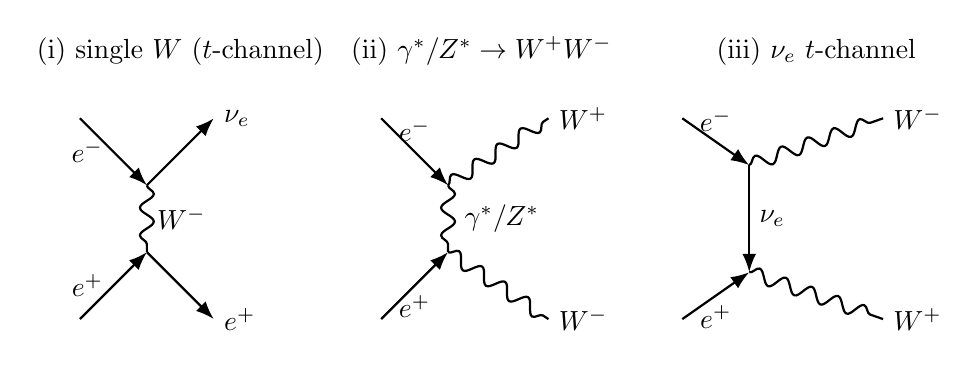
\begin{tikzpicture}[scale=0.85,>=Latex]
% (i) single W
\node at (-4.5,2.5) {(i) single $W$ ($t$-channel)};
\draw[->,thick](-6,1.5)--(-5,0.5)node[midway,left]{$e^-$};
\draw[->,thick](-5,0.5)--(-4,1.5)node[right]{$\nu_e$};
\draw[decorate,decoration={snake},thick](-5,0.5)--(-5,-0.5)node[midway,right]{$W^-$};
\draw[->,thick](-6,-1.5)--(-5,-0.5)node[midway,left]{$e^+$};
\draw[->,thick](-5,-0.5)--(-4,-1.5)node[right]{$e^+$};
% (ii) WW via gamma/Z
\node at (0,2.5) {(ii) $\gamma^*/Z^*\to W^+W^-$};
\draw[->,thick](-1.5,1.5)--(-0.5,0.5)node[midway,above]{$e^-$};
\draw[->,thick](-1.5,-1.5)--(-0.5,-0.5)node[midway,below]{$e^+$};
\draw[decorate,decoration={snake},thick](-0.5,0.5)--(-0.5,-0.5);
\node[right] at (-0.4,0) {$\gamma^*/Z^*$};
\draw[decorate,decoration={snake},thick](-0.5,0.5)--(1,1.5)node[right]{$W^+$};
\draw[decorate,decoration={snake},thick](-0.5,-0.5)--(1,-1.5)node[right]{$W^-$};
% (iii) WW via nu_e
\node at (5,2.5) {(iii) $\nu_e$ $t$-channel};
\draw[->,thick](3,1.5)--(4,0.8)node[midway,above]{$e^-$};
\draw[->,thick](4,0.8)--(4,-0.8)node[midway,right]{$\nu_e$};
\draw[->,thick](3,-1.5)--(4,-0.8)node[midway,below]{$e^+$};
\draw[decorate,decoration={snake},thick](4,0.8)--(6,1.5)node[right]{$W^-$};
\draw[decorate,decoration={snake},thick](4,-0.8)--(6,-1.5)node[right]{$W^+$};
\end{tikzpicture}
\end{center}

\subsection*{(b) $W$ decay modes and detector signatures}

The charged current of the SM gives the $W$ a universal coupling to each weak doublet,
weighted by colour. The branching fractions are approximately
\begin{equation}
\mathrm{BR}(W^+\to e^+\nu_e)=\mathrm{BR}(\mu^+\nu_\mu)=\mathrm{BR}(\tau^+\nu_\tau)\simeq 11\%,\qquad \mathrm{BR}(W^+\to q\bar q')\simeq 67\%,
\end{equation}
where the hadronic modes are $u\bar d$ and $c\bar s$ (with small CKM-mixed contributions
to $u\bar s$, $c\bar d$, etc., and $W\to t b$ kinematically forbidden). The factor of 3
enhancement in the hadronic mode comes from colour.

\textit{Detection signatures in a hermetic $4\pi$ detector:}
\begin{itemize}
\item $W\to e\nu_e$: a single high-$p_T$ isolated electromagnetic shower (matched
track + ECAL deposit) plus large missing transverse momentum (the neutrino) carrying away
$\sim M_W/2$ of energy.
\item $W\to \mu\nu_\mu$: a single high-$p_T$ isolated muon track penetrating to the muon
chambers, leaving minimum-ionising signals throughout the calorimeter, plus large missing
transverse momentum.
\item $W\to \tau\nu_\tau$: the $\tau$ decays before reaching tracking, giving either a
narrow ``1-prong'' or ``3-prong'' track jet in the tracker, low charged-particle multiplicity,
significant missing energy from one or two neutrinos. About $35\%$ of $\tau$'s decay
leptonically (giving an $e$ or $\mu$ + missing energy), the rest hadronically.
\item $W\to q\bar q'$: two collimated hadronic jets back-to-back in the $W$ rest frame
(boosted in the lab), each with charged tracks and ECAL+HCAL deposits, total invariant
mass $\simeq M_W$, no missing energy. With $b$- or $c$-tagging the $cs$ mode can be
identified by a displaced secondary vertex.
\end{itemize}

\subsection*{(c) Relativistic Breit--Wigner}

\paragraph{(i) Definitions.} In
\begin{equation}
\sigma(E)=\frac{\alpha\,\Gamma_i\Gamma_f}{(E^2-M^2)^2+M^2\Gamma^2},
\label{eq:rel-BW}
\end{equation}
$E$ is the c.m.~total energy ($\sqrt s$), $M$ the resonance pole mass, $\Gamma$ its total
decay width (so $1/\Gamma$ is its mean proper lifetime), $\Gamma_i$ the partial width into
the initial-state channel and $\Gamma_f$ into the observed final state. The constant
$\alpha$ collects spin-counting and unitarity factors,
\begin{equation}
\alpha = \frac{12\pi}{p_i^2}\,\frac{2J+1}{(2s_1+1)(2s_2+1)},
\label{eq:alpha-BW}
\end{equation}
so $\alpha$ depends on the c.m.~momentum $p_i$ of the initial-state particles, on the
resonance spin $J$ and on the spins $s_{1,2}$ of the two colliding particles.

\paragraph{(ii) Non-relativistic limit.} Near the resonance write $E=M+\varepsilon$ with
$\varepsilon\ll M$. Then
\begin{equation}
E^2-M^2=(E-M)(E+M)\simeq 2M\varepsilon,
\label{eq:near-res-num}
\end{equation}
so the denominator becomes
\begin{equation}
(E^2-M^2)^2+M^2\Gamma^2\simeq 4 M^2\varepsilon^2 + M^2\Gamma^2 = 4M^2\!\left[\varepsilon^2+(\Gamma/2)^2\right].
\label{eq:near-res-denom}
\end{equation}
Substituting into~\eqref{eq:rel-BW},
\begin{equation}
\sigma(E)\simeq \frac{\alpha\,\Gamma_i\Gamma_f}{4 M^2}\,\frac{1}{(E-M)^2+(\Gamma/2)^2}.
\label{eq:NR-BW}
\end{equation}
Using $\alpha=12\pi(2J+1)/[p_i^2(2s_1+1)(2s_2+1)]$ and noting that
$p_i^2\simeq (M/2)^2\cdot v^2_\mathrm{rel}\to$ for non-relativistic colliding particles
$p_i^2 = \mu^2 v^2 \to$ in fact one must be careful: the standard form recovers the textbook
\emph{non-relativistic} Breit--Wigner,
\begin{equation}
\boxed{\;\sigma(E)=\frac{\pi}{k^2}\,\frac{(2J+1)}{(2s_1+1)(2s_2+1)}\,\frac{\Gamma_i\Gamma_f}{(E-M)^2+(\Gamma/2)^2},\;}
\label{eq:NR-BW-final}
\end{equation}
which is the celebrated Breit--Wigner formula. The replacement $4M^2\to 1/(\hbar^2\,\text{something})$
follows from the kinematic identification of the c.m.~wavenumber $k=p_i/\hbar$.

\subsection*{(d) The $e^+e^-\to$\,hadrons cross section}

\paragraph{(i) Identification of resonances $a$--$f$.}
Reading the cross section in order of increasing $\sqrt s$:
\begin{itemize}
\item \textbf{$a$ ($\sim 0.78$\,GeV):} the $\rho(770)/\omega(782)$ doublet --- light vector
mesons made of $u\bar u$ and $d\bar d$ ($I=1$ and $I=0$ respectively), strongly produced
through one-photon annihilation $e^+e^-\to\gamma^*\to V$.
\item \textbf{$b$ ($\sim 1.02$\,GeV):} the $\phi(1020)$, a nearly pure $s\bar s$ vector
meson; its width is small ($\sim 4$\,MeV) because OZI rule suppresses its dominant decay
into non-strange hadrons.
\item \textbf{$c$ ($\sim 3.1$\,GeV):} the $J/\psi$, the $1\,^3S_1$ state of the
$c\bar c$ system (charmonium); narrow ($\Gamma\simeq 93$\,keV) again by the OZI rule
because $M_{J/\psi}<2M_D$.
\item \textbf{$d$ ($\sim 3.7$\,GeV):} the $\psi(3686)$ (a.k.a.~$\psi'$, $2\,^3S_1$
charmonium); narrow because still below $D\bar D$ threshold ($2M_D\simeq 3.74$\,GeV). The
``open-charm'' threshold lies just above this peak.
\item \textbf{$e$ ($\sim 9.5$\,GeV):} the $\Upsilon(1S)$ ($b\bar b$ vector), and its
radial excitations $\Upsilon(2S)$, $\Upsilon(3S)$ all below $B\bar B$ threshold; very narrow.
\item \textbf{$f$ ($\sim 91$\,GeV):} the $Z^0$ boson, electroweak resonance produced by
$e^+e^-\to Z^*$, with mass $M_Z=91.19$\,GeV and width $\Gamma_Z\simeq 2.5$\,GeV.
\end{itemize}

\paragraph{(ii) Overall slope and discontinuity near $d$.}
Off resonance the cross section is dominated by the QED process $e^+e^-\to\gamma^*\to q\bar q$,
which gives
\begin{equation}
\sigma(e^+e^-\to q\bar q)=\frac{4\pi\alpha^2}{3 s}\,N_c\sum_q Q_q^2,
\label{eq:R-cross-section}
\end{equation}
falling as $1/s$ --- this is the overall declining slope. The discontinuity near $d$ at
$\sqrt s\simeq 2 M_D \simeq 3.74$\,GeV is the opening of the open-charm production
threshold: above this energy a new pair of quark flavours ($c\bar c$ giving $D\bar D$ etc.)
becomes kinematically accessible, so the sum $\sum_q Q_q^2$ jumps from $u,d,s$ contributions
($Q^2=4/9+1/9+1/9=2/3$) to $u,d,s,c$ contributions ($+4/9$, total $10/9$), causing a step
upward in the smooth continuum. The familiar $R$-ratio $R=\sigma(\mathrm{had})/\sigma(\mu\mu)
= N_c\sum Q_q^2$ accordingly steps from $2$ to $10/3$.

\paragraph{(iii) Width of peaks $a$ and $f$.}
The width of a resonance is set by the inverse lifetime via $\Gamma=\hbar/\tau$. Peaks $a$
($\rho/\omega$) and $f$ ($Z^0$) are broad for opposite reasons.

The $\rho^0$ has width $\Gamma_\rho\simeq 150$\,MeV because it decays \emph{strongly} into
two pions ($\rho^0\to\pi^+\pi^-$ has BR $\simeq 100\%$), and strong decays proceed on
$\tau\sim 1/\Lambda_\mathrm{QCD}\sim 10^{-23}$\,s, giving the broadest possible widths.
The decay channel is kinematically wide open ($M_\rho\gg 2 m_\pi$) and OZI-allowed.

The $Z^0$ has width $\Gamma_Z\simeq 2.5$\,GeV because, although mediated by the weak
interaction, the available phase space is enormous: the $Z$ decays into all kinematically
accessible $f\bar f$ pairs --- three charged leptons, three neutrino flavours, and five
quark flavours times three colours --- and each channel contributes comparable partial
width. Equivalently, $\Gamma_Z\propto G_F M_Z^3\sum N_c(g_V^2+g_A^2)$, and the cube of the
mass scale ($M_Z^3$) makes the absolute width large despite the small electroweak coupling.
A separate, observational, broadening mechanism for the $Z$ peak measured at $e^+e^-$
colliders is the initial-state photon radiation: each beam emits collinear photons before
annihilating, smearing the effective $\sqrt s$ distribution and broadening the apparent
peak.

\section*{Question 3 --- Beta decay, weak cross section, and double beta decay}

\textbf{Problem statement.} Required: leading-order quark-level diagrams for $\beta$-decay
and inverse $\beta$-decay; a Pontecorvo dimensional estimate of the inverse-$\beta$-decay
cross section at 1\,MeV; its energy dependence and threshold; the assumptions and term
structure of the SEMF; identification of which SEMF feature drives double-$\beta$ decay; an
estimate of $Q$ for $^{130}$Te double-$\beta$ decay; the SM symmetries that forbid massless
$\nu\to\bar\nu$ conversion; the form of the $0\nu\beta\beta$ half-life; and a 90\% C.L. upper
bound on $m_{\beta\beta}$ given a one-tonne-year null exposure.

\subsection*{(a) $\beta$-decay and inverse $\beta$-decay diagrams}

In the quark picture $\beta^-$ decay of a free neutron is mediated by a $W^-$ that converts
a $d$-quark to a $u$-quark and decays leptonically to $e^-\bar\nu_e$. ``Inverse'' $\beta$
decay $\bar\nu_e+p\to n+e^+$ is the same vertex run with a $W$ exchanged between the
hadronic and leptonic currents in $s$- or $t$-channel; the $\bar\nu_e$ line is incoming and
the $e^+$ is outgoing.

\begin{center}
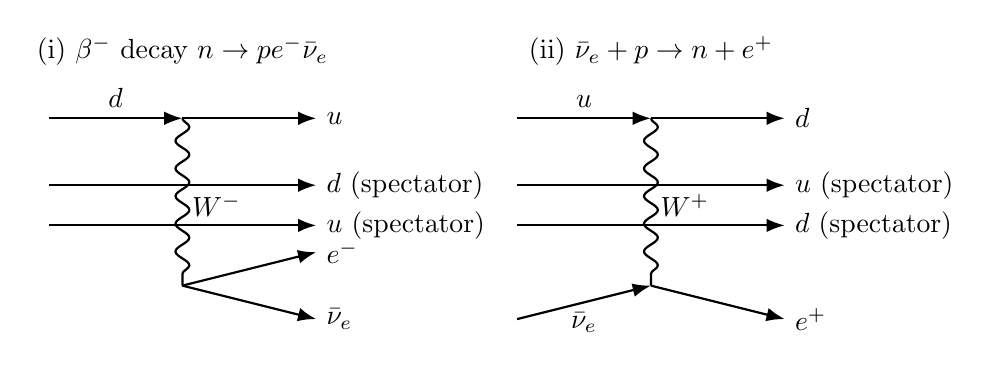
\begin{tikzpicture}[scale=0.85,>=Latex]
\node at (-3,3) {(i) $\beta^-$ decay $n\to p e^-\bar\nu_e$};
\draw[->,thick] (-5,2)--(-3,2) node[midway,above]{$d$};
\draw[->,thick] (-3,2)--(-1,2) node[right]{$u$};
\draw[->,thick] (-5,1)--(-1,1) node[right]{$d$ (spectator)};
\draw[->,thick] (-5,0.4)--(-1,0.4) node[right]{$u$ (spectator)};
\draw[decorate,decoration={snake},thick] (-3,2)--(-3,-0.5);
\node[right] at (-3,0.7) {$W^-$};
\draw[->,thick] (-3,-0.5)--(-1,0)node[right]{$e^-$};
\draw[->,thick] (-3,-0.5)--(-1,-1) node[right]{$\bar\nu_e$};
% inverse
\node at (4,3) {(ii) $\bar\nu_e+p\to n+e^+$};
\draw[->,thick] (2,2)--(4,2) node[midway,above]{$u$};
\draw[->,thick] (4,2)--(6,2) node[right]{$d$};
\draw[->,thick] (2,1)--(6,1) node[right]{$u$ (spectator)};
\draw[->,thick] (2,0.4)--(6,0.4) node[right]{$d$ (spectator)};
\draw[decorate,decoration={snake},thick] (4,2)--(4,-0.5);
\node[right] at (4,0.7) {$W^+$};
\draw[->,thick] (2,-1)--(4,-0.5) node[midway,below]{$\bar\nu_e$};
\draw[->,thick] (4,-0.5)--(6,-1) node[right]{$e^+$};
\end{tikzpicture}
\end{center}

The two diagrams share the same $W$-boson exchange vertex; ``crossing'' the $\bar\nu_e$
line from outgoing to incoming and reversing the leptonic charge transforms one into the
other. They are related by detailed balance and CPT.

\subsection*{(b) Pontecorvo cross section estimate}

\paragraph{(i) Cross section at 1\,MeV.} The neutron lifetime $\tau_n\simeq 880$\,s sets the
weak decay rate. By time-reversal symmetry the same matrix element appears in inverse
$\beta$-decay. A 1\,MeV anti-neutrino has reduced de Broglie wavelength
\begin{equation}
\lambdabar = \hbar/p_\nu = \hbar c/(E_\nu) = \frac{197\,\mathrm{MeV\,fm}}{1\,\mathrm{MeV}}=197\,\mathrm{fm}.
\label{eq:lambda}
\end{equation}
The neutrino traversing a proton has the wavepacket overlapping the proton for a transit
time
\begin{equation}
\Delta t \sim \lambdabar/c.
\label{eq:transit}
\end{equation}
Within that interaction time the probability for the weak vertex to fire is
$P\sim \Delta t/\tau_n$. Geometrically the relevant cross-sectional area is $\sim\pi\lambdabar^2$
(one-particle quantum scattering geometry), so the effective cross section is
\begin{equation}
\sigma\sim \pi\lambdabar^2 \cdot P=\pi\lambdabar^2 \cdot \frac{\lambdabar}{c\tau_n}.
\label{eq:pontecorvo}
\end{equation}
In SI/natural units, with $\lambdabar=1.97\times 10^{-13}$\,m and $c\tau_n=2.64\times 10^{11}$\,m,
\begin{equation}
\sigma\sim \pi\frac{\lambdabar^3}{c\tau_n}=\pi\,\frac{(1.97\times 10^{-13})^3}{2.64\times 10^{11}}\,\mathrm{m^2}
\simeq 9\times 10^{-50}\,\mathrm{m^2}\simeq 10^{-44}\,\mathrm{cm^2}.
\label{eq:numeric}
\end{equation}
This is in spectacular agreement with the measured low-energy inverse-$\beta$ cross section
of $\sim 10^{-43}\,\mathrm{cm^2}$ at a few MeV.

\paragraph{(ii) Energy dependence.}
At higher energies $\lambdabar=\hbar c/E_\nu$ shrinks as $1/E_\nu$, so
$\sigma\propto \lambdabar^3\propto 1/E_\nu^3$? No --- this would be wrong because we have
not separated phase-space factors. The more careful Pontecorvo argument keeps the matrix
element fixed and writes the rate as the product of (i) a final-state phase-space factor
$\propto p_e E_e\propto E_\nu^2$ for the relativistic outgoing electron at high energies,
and (ii) a flux factor $1/v_\nu$. Equivalently, dimensional analysis at high energies (still
below the $W$ pole) gives
\begin{equation}
\sigma\propto G_F^2\,s\sim G_F^2\,E_\nu^2,
\label{eq:cross-rises}
\end{equation}
because $G_F$ has dimension $[\text{energy}]^{-2}$. Thus
\begin{equation}
\boxed{\,\sigma_\mathrm{IBD}(E_\nu)\propto E_\nu^2\,}
\label{eq:e2-rise}
\end{equation}
above threshold and below $\sqrt s\sim M_W$. (For $\sqrt s\gtrsim M_W$ the propagator
$1/(q^2-M_W^2)$ stops being constant and the cross section saturates.)

\paragraph{(iii) Threshold for $\bar\nu_e p\to n e^+$.}
Energy--momentum conservation in the lab where the proton is at rest gives at threshold,
when neutron and positron are at rest in the c.m.~frame,
\begin{equation}
s_\mathrm{thresh}=(m_n+m_e)^2 c^4 = (E_\nu+m_p c^2)^2-(E_\nu)^2,
\label{eq:thresh-s}
\end{equation}
treating the neutrino as massless ($p_\nu c=E_\nu$). Expanding,
\begin{equation}
(m_n+m_e)^2 c^4=2 E_\nu m_p c^2 + m_p^2 c^4,
\label{eq:thresh-expand}
\end{equation}
so
\begin{equation}
E_\nu^\mathrm{thresh}=\frac{(m_n+m_e)^2 - m_p^2}{2 m_p}\,c^2 = \frac{(m_n-m_p)(m_n+m_p)+2 m_e(m_n+m_e)+m_e^2}{2 m_p}c^2.
\label{eq:thresh-result}
\end{equation}
Numerically with $m_n-m_p=1.293$\,MeV/$c^2$, $m_e=0.511$\,MeV/$c^2$ and $m_p=938.3$\,MeV/$c^2$,
\begin{equation}
\boxed{\,E_\nu^\mathrm{thresh}\simeq (m_n-m_p)c^2+m_e c^2 + \frac{(m_n-m_p)^2 + m_e^2 + 2m_e(m_n-m_p)}{2 m_p}c^2 \simeq 1.806\,\mathrm{MeV}.\,}
\label{eq:thresh-val}
\end{equation}
Approximately, $E_\nu^\mathrm{thresh}\simeq (m_n+m_e-m_p)c^2 = 1.804$\,MeV plus a tiny
recoil correction $\sim m_e^2/m_p c^2\simeq 0.0014$\,MeV.

\subsection*{(c) SEMF: assumptions and terms}

The liquid-drop model treats the nucleus as an incompressible fluid of nucleons of
constant density (saturating nuclear matter). The main assumptions are: (i) nucleons
attract via short-range, charge-independent forces saturating at nearest neighbours; (ii)
nuclear matter is essentially incompressible, so the nuclear volume $V\propto A$ and the
radius $R=r_0 A^{1/3}$; (iii) the Coulomb force between protons is the only long-range
interaction; (iv) shell-structure / quantum-mechanical effects appear only as the asymmetry
and pairing terms.

The five terms in
\begin{equation}
\mathrm{BE}(A,Z)=a_V A - a_S A^{2/3}-a_C\frac{Z(Z-1)}{A^{1/3}}-a_A\frac{(A-2Z)^2}{A}+\delta
\label{eq:SEMF}
\end{equation}
have the following physical origin:
\begin{itemize}
\item \textit{Volume term} $a_V A$: each nucleon binds with a roughly fixed number of
neighbours, contributing a constant binding $\sim a_V\simeq 15.75$\,MeV per nucleon.
\item \textit{Surface term} $-a_S A^{2/3}$: nucleons on the surface have fewer neighbours,
analogous to surface tension of a liquid drop; the surface area scales as $R^2\propto A^{2/3}$.
\item \textit{Coulomb term} $-a_C Z(Z-1)/A^{1/3}$: classical electrostatic energy of $Z$
protons distributed uniformly in a sphere of radius $R\propto A^{1/3}$; pairs of protons
$Z(Z-1)/2$.
\item \textit{Asymmetry term} $-a_A(A-2Z)^2/A$: a quantum effect from the Pauli principle
favouring $N=Z$, since for a fixed $A$ filling separate $n$ and $p$ Fermi seas to equal
heights minimises the total kinetic energy.
\item \textit{Pairing term} $\delta=\pm 11.18/\sqrt A$ (or zero): another quantum effect
favouring even $Z$ and even $N$ (where like-spin nucleons pair into $J=0$ pairs giving
extra binding).
\end{itemize}

\subsection*{(d) Double-$\beta$ decay and the $Q$-value of $^{130}$Te}

The pairing term $\delta$ is responsible. For an even-even nucleus, the SEMF gives a more
deeply bound parabola in $Z$ at fixed $A$ than for odd-odd nuclei: the even-even and
odd-odd mass parabolas are offset by $2\delta=22.4/\sqrt A$\,MeV. A nucleus that would have
to pass through an odd-odd intermediate to $\beta$-decay can therefore be \emph{stable}
against single $\beta$ decay (the intermediate is heavier) yet \emph{unstable} against
direct double-$\beta$ decay to the lighter even-even daughter at $Z+2$. $^{130}$Te is one
such case; the chain $^{130}_{52}\mathrm{Te}\to {}^{130}_{53}\mathrm{I}$ is energetically
forbidden, but $^{130}_{52}\mathrm{Te}\to{}^{130}_{54}\mathrm{Xe}$ is allowed.

The $Q$-value is
\begin{equation}
Q_{\beta\beta}=\left[M(A,Z)-M(A,Z+2)-2 m_e\right]c^2.
\label{eq:Q-double}
\end{equation}
Computing $\Delta\mathrm{BE}$ between the two even-even nuclei from the SEMF, the volume,
surface and asymmetry terms are unchanged ($A$ and $|A-2Z|$ are nearly the same; for $A=130$,
moving from $Z=52$ to $Z=54$ changes $(A-2Z)^2/A$ from $26^2/130=5.2$ to $22^2/130=3.72$,
$\Delta=1.48$, $a_A\Delta=35.1$\,MeV \emph{gain}); the Coulomb term grows by
\begin{equation}
\Delta E_C = a_C \frac{Z'(Z'-1)-Z(Z-1)}{A^{1/3}} = 0.711\,\frac{54\cdot 53 - 52\cdot 51}{130^{1/3}}=0.711\cdot\frac{210}{5.066}=29.4\,\mathrm{MeV},
\label{eq:Coulomb-step}
\end{equation}
which costs binding (the Coulomb term enters with a minus sign, so going to higher $Z$
\emph{reduces} BE by $29.4$\,MeV). Pairing $\delta$ is unchanged (both even-even). Adding
asymmetry gain ($+35.1$\,MeV) and Coulomb loss ($-29.4$\,MeV) gives a SEMF prediction
\begin{equation}
Q_{\beta\beta}^\mathrm{SEMF}\simeq 35.1-29.4 - 2 m_e c^2 - (m_n-m_p\text{ corrections})\simeq 5.7-2(0.511)\simeq -0.3\,\mathrm{MeV}.
\label{eq:Q-naive}
\end{equation}
Adding the question's stated correction of $+6.5$\,MeV (the SEMF underestimates by this
much for $^{130}$Te due to shell effects beyond the liquid-drop approximation),
\begin{equation}
\boxed{\,Q_{\beta\beta}(^{130}\mathrm{Te})\simeq 0.3\text{--}6.5+6.5\simeq 2.5\,\mathrm{MeV}\,}\quad\text{(measured value 2.527\,MeV).}
\label{eq:Q-Te-final}
\end{equation}
Within the precision of a back-of-envelope SEMF the value is comfortably consistent with
the experimental endpoint $Q_{\beta\beta}=2.527$\,MeV.

\subsection*{(e) Justification of the $0\nu\beta\beta$ half-life formula}

In the SM, lepton number $L$ is exactly conserved (a global accidental symmetry), and
massless neutrinos have a definite chirality: the neutrino is purely left-handed
($P_L\nu=\nu$) and the antineutrino purely right-handed. Conversion of $\nu$ to $\bar\nu$
would require both $\Delta L=2$ violation and a chirality flip --- the first is impossible
in the SM, the second impossible for a massless particle. If neutrinos are Majorana
\emph{and} massive, both obstructions are lifted: the Majorana mass term is $L$-violating
($\Delta L=2$) and the mass itself provides the chirality flip with amplitude $\sim m_\nu/E_\nu$.

The half-life is the inverse rate, and Fermi's Golden Rule gives
$\Gamma\propto |\mathcal M|^2\times(\text{phase space})$. The amplitude factorises into a
nuclear matrix element $M^{0\nu}$ describing the transition of the parent nucleus to the
daughter via two simultaneous $W$-vertices, and an elementary leptonic factor proportional
to $m_{\beta\beta}$ (the Majorana mass insertion required to flip the neutrino chirality
between the two $W$ vertices). Squaring gives
$\Gamma\propto |M^{0\nu}|^2 m_{\beta\beta}^2$, and the available phase space for the two
outgoing electrons defines $G^{0\nu}$. Hence
\begin{equation}
\boxed{\;(T^{0\nu}_{1/2})^{-1}=G^{0\nu}|M^{0\nu}|^2 m_{\beta\beta}^2.\;}
\label{eq:T0nu}
\end{equation}

\subsection*{(f) 90\% C.L. upper bound on $m_{\beta\beta}$}

\textit{Number of $^{130}$Te atoms in 1 tonne.}
\begin{equation}
N=\frac{10^6\,\mathrm{g}}{130\,\mathrm{g/mol}}\,N_A=\frac{10^6}{130}\cdot 6.022\times 10^{23}=4.63\times 10^{27}\;\text{atoms}.
\label{eq:N-atoms}
\end{equation}

\textit{Poisson upper limit.} For zero observed events with no background, the 90\%
confidence upper limit on the expected number of events is
$\mu_\mathrm{up}=-\ln(1-0.90)=2.303$.

\textit{Translating to a half-life lower bound.} The number of decays in time $t$ is
$N_\mathrm{dec}=N\,t/\tau = N t\ln 2/T_{1/2}$. With $t=1\,\mathrm{yr}$,
\begin{equation}
T_{1/2}^{0\nu}>\frac{N\,t\,\ln 2}{\mu_\mathrm{up}}=\frac{4.63\times 10^{27}\cdot 1\,\mathrm{yr}\cdot 0.693}{2.303}=1.39\times 10^{27}\,\mathrm{yr}.
\label{eq:T-bound}
\end{equation}

\textit{Translating to a mass bound.} From \eqref{eq:T0nu},
$m_{\beta\beta}^2=1/[T_{1/2}^{0\nu}\,G^{0\nu}\,|M^{0\nu}|^2]$. With $G^{0\nu}=5.5\times 10^{-15}$\,yr$^{-1}$
and $|M^{0\nu}|=4$,
\begin{equation}
m_{\beta\beta}^2 < \frac{1}{1.39\times 10^{27}\cdot 5.5\times 10^{-15}\cdot 16}=\frac{1}{1.22\times 10^{14}}=8.2\times 10^{-15}.
\label{eq:m-sq}
\end{equation}
Recalling that $m_{\beta\beta}$ is in units of $m_e c^2=0.511$\,MeV,
\begin{equation}
m_{\beta\beta} < \sqrt{8.2\times 10^{-15}}\;m_e c^2 = 9.05\times 10^{-8}\cdot 0.511\,\mathrm{MeV}=4.6\times 10^{-8}\,\mathrm{MeV}.
\label{eq:mbb}
\end{equation}
\begin{equation}
\boxed{\;m_{\beta\beta}<46\,\mathrm{meV}\quad\text{at 90\% C.L.}\;}
\label{eq:mbb-final}
\end{equation}
This is in the same ballpark as the leading current experimental limits from CUORE/KamLAND-Zen.

\section*{Question 4 --- Cross sections, Born approximation, and neutron moderation}

\textbf{Problem statement.} Required: a derivation of the cross-section formula
$\sigma=R_S V/(N N_T v)$ from a thin-block geometry, identification of the Fermi
golden-rule rate; the exponential attenuation through a thick block; the Born-approximation
differential cross section for a square-well potential, with constants $A$ and $B$
determined; the low-energy total cross section in the form $4\pi R^2$; and a sequence of
neutron-moderation results in graphite (mean post-collision energy, mean number of
collisions to thermalise, mean free time, and total thermalisation time).

\subsection*{(a) Cross-section bookkeeping}

\paragraph{(i) From counts to $\sigma$.} The block contains $N_T$ targets in a volume
$V=A\de x$, so the number density is $n_T=N_T/V$. The flux of incoming particles is
$\Phi=N/(A\,\de t)$. Each target presents an effective area $\sigma$, so the total
``blocked area'' seen by an incoming particle is $N_T\sigma$. The probability that any one
incoming particle scatters in traversing the slab is $P_\mathrm{scatt}=N_T\sigma/A$. Hence
the number of scattering events in time $\de t$ is
\begin{equation}
\de N_\mathrm{scatt}=N\cdot \frac{N_T\sigma}{A},
\label{eq:dN-scatt}
\end{equation}
and the scattering rate is $R_S\equiv\de N_\mathrm{scatt}/\de t$. Now $\de t=\de x/v$, where
$v$ is the speed of an incoming projectile (the relative velocity in the target rest frame).
Substituting and rearranging,
\begin{equation}
R_S = \frac{N\,N_T\,\sigma}{A}\cdot\frac{v}{\de x}=\frac{N N_T\sigma\,v}{V}\;\Longrightarrow\;
\boxed{\;\sigma=\frac{R_S V}{N N_T v}.\;}
\label{eq:sigma-counts}
\end{equation}

The variable $v$ is the speed of an individual beam particle (equivalently, the magnitude
of the relative velocity between projectile and target, since in this problem the targets
are at rest). The numerator $R_S$ is the experimentally observed scattering rate; the
denominator factor $\Phi=N/(A\de t)\propto Nv/V\cdot(\text{stuff})$ encodes the flux. The
piece of the formula that is in principle calculable from the Fermi golden rule is the
\emph{rate per target per beam particle}, $W_{i\to f}=R_S/(N N_T)$, which by Fermi's golden
rule is $W=(2\pi/\hbar)|\langle f|V|i\rangle|^2\rho(E_f)$.

\paragraph{(ii) Thick block.} For a thick block divide it into infinitesimal slabs of
thickness $\de x$ in which a fraction
$\de N/N=-(N_T\sigma/A_\mathrm{slab})=-n_T\sigma\,\de x$ scatters out of the beam. Hence
\begin{equation}
\frac{\de N(x)}{\de x}=-n_T\sigma\, N(x)\;\Longrightarrow\; N(x)=N_0\,e^{-n_T\sigma\,x}.
\label{eq:beer-lambert}
\end{equation}
The number of scattered particles emerging from a slab of length $x$ is therefore
\begin{equation}
N_\mathrm{scatt}=N_0-N(x)=N_0\left[1-e^{-n_T\sigma\,x}\right]=N\bigl[1-e^{\alpha}\bigr]\quad\text{with}\quad
\boxed{\;\alpha = -n_T\sigma\,x = -\frac{N_T\sigma\,x}{V}.\;}
\label{eq:alpha}
\end{equation}
Equivalently $\alpha=-x/\lambda$ with $\lambda=1/(n_T\sigma)$ the mean free path.

\subsection*{(b) Born approximation for a spherical square well}

\paragraph{(i) Differential cross section.} The first-order Born approximation gives the
scattering amplitude as the Fourier transform of the potential,
\begin{equation}
f(\mathbf q)=-\frac{2\mu}{\hbar^2 q^2}\int_0^\infty V(r)\,\sin(qr)\, q r\,\de r\cdot\frac{2}{q}=-\frac{2\mu}{\hbar^2 q}\int_0^\infty V(r)\,r\sin(qr)\,\de r,
\label{eq:Born-general}
\end{equation}
where $\mathbf q=\mathbf k_f-\mathbf k_i$ has magnitude $q=2k\sin(\theta/2)$ and
$\mu$ is the reduced mass. For $V(r)=-V_0\,\Theta(a-r)$ this becomes
\begin{equation}
f(q)=\frac{2\mu V_0}{\hbar^2 q}\int_0^a r\sin(qr)\,\de r.
\label{eq:Born-step1}
\end{equation}
Integrating by parts ($u=r$, $\de v=\sin(qr)\de r$),
\begin{equation}
\int_0^a r\sin(qr)\,\de r=\left[-\frac{r\cos(qr)}{q}\right]_0^a+\frac{1}{q}\int_0^a\cos(qr)\,\de r=-\frac{a\cos(qa)}{q}+\frac{\sin(qa)}{q^2},
\label{eq:integral}
\end{equation}
so
\begin{equation}
f(q)=\frac{2\mu V_0}{\hbar^2 q}\cdot\frac{1}{q^2}\bigl[\sin(qa)-q a\cos(qa)\bigr]=\frac{2\mu V_0}{\hbar^2 q^3}\bigl[\sin(qa)-qa\cos(qa)\bigr].
\label{eq:f-of-q}
\end{equation}
The differential cross section is
\begin{equation}
\frac{\de\sigma}{\de\Omega}=|f(q)|^2 = \frac{4\mu^2 V_0^2}{\hbar^4 q^6}\bigl[\sin(qa)-qa\cos(qa)\bigr]^2.
\label{eq:dsig-Born}
\end{equation}
Comparing with the form $A[\sin(qa)-B\cos(qa)]^2$,
\begin{equation}
\boxed{\;A=\frac{4\mu^2 V_0^2}{\hbar^4 q^6}\,, \qquad B = qa.\;}
\label{eq:AB}
\end{equation}

\paragraph{(ii) Low-energy limit.} For $ka\ll 1$ the momentum transfer $q=2k\sin(\theta/2)\le 2k$ is also small, so $qa\ll 1$ and we expand
\begin{equation}
\sin(qa)-qa\cos(qa)=\Bigl(qa-\tfrac{(qa)^3}{6}+\cdots\Bigr)-qa\Bigl(1-\tfrac{(qa)^2}{2}+\cdots\Bigr)=\tfrac{(qa)^3}{3}+\mathcal O((qa)^5).
\label{eq:expand}
\end{equation}
Substituting into~\eqref{eq:dsig-Born},
\begin{equation}
\frac{\de\sigma}{\de\Omega}=\frac{4\mu^2 V_0^2}{\hbar^4 q^6}\cdot\frac{(qa)^6}{9}=\frac{4\mu^2 V_0^2 a^6}{9\hbar^4}.
\label{eq:isotropic}
\end{equation}
The differential cross section is independent of angle ($s$-wave isotropy), as it must be
in the low-energy limit. Integrating over the full solid angle $4\pi$,
\begin{equation}
\sigma_\mathrm{tot}=4\pi\cdot\frac{4\mu^2 V_0^2 a^6}{9\hbar^4}=4\pi R^2\quad\text{with}\quad
\boxed{\;R=\frac{2\mu V_0 a^3}{3\hbar^2}.\;}
\label{eq:R-low-E}
\end{equation}
Physically $R$ is the (Born) scattering length of the well; the cross section
$4\pi R^2$ is the standard textbook low-energy scattering result.

\subsection*{(c) Neutron moderation in graphite}

\paragraph{(i) Mean post-collision energy.} In the c.m.~frame the elastic scattering is
isotropic by assumption. The lab-frame final neutron energy at scattering angle $\theta^*$
in the c.m.~frame is, by standard kinematics for elastic scattering of mass $m_n$ on a
target $M$ at rest in the lab,
\begin{equation}
E_\mathrm{lab}=E_0\,\frac{1+\alpha+(1-\alpha)\cos\theta^*}{2}, \quad \alpha\equiv\left(\frac{M-m_n}{M+m_n}\right)^2.
\label{eq:elastic-kin}
\end{equation}
This is obtained by Lorentz-boosting the post-scatter neutron from the c.m.~frame (where it
has the same speed as before scattering) back to the lab. The c.m.~speed is
$V_\mathrm{cm}=m_n v_0/(M+m_n)$, where $v_0$ is the initial lab-frame neutron speed; the
neutron's speed in the c.m.~frame is $u=Mv_0/(M+m_n)$. After scattering by $\theta^*$ in the
c.m.~frame the neutron's lab-frame energy is
$\tfrac12 m_n(V_\mathrm{cm}^2+u^2+2 V_\mathrm{cm}u\cos\theta^*)$, which evaluates to the
expression above.

Averaging over isotropic c.m.~angles, $\langle\cos\theta^*\rangle=0$, hence
\begin{equation}
\langle E\rangle = E_0\,\frac{1+\alpha}{2}=\frac{E_0}{2}\left[1+\left(\frac{M-m_n}{M+m_n}\right)^2\right].
\label{eq:E-avg-1}
\end{equation}
Expanding the square,
\begin{equation}
1+\left(\frac{M-m_n}{M+m_n}\right)^2=\frac{(M+m_n)^2+(M-m_n)^2}{(M+m_n)^2}=\frac{2(M^2+m_n^2)}{(M+m_n)^2},
\label{eq:expand-alpha}
\end{equation}
so
\begin{equation}
\boxed{\;\langle E\rangle = \frac{M^2+m_n^2}{(M+m_n)^2}\,E_0 \equiv \alpha' E_0,\;}
\label{eq:E-avg-final}
\end{equation}
matching the form quoted in the question (with the question's $\alpha$ being our
$\alpha'=(M^2+m_n^2)/(M+m_n)^2$, distinct from the conventional $\alpha=(M-m_n)^2/(M+m_n)^2$).

For $M=12 m_n$, $\alpha' = (144+1)/169 = 145/169 \simeq 0.858$. So each collision retains
$\sim 86\%$ of the neutron's energy on average.

\paragraph{(ii) Number of collisions to thermalise.} After $n$ collisions
$E_n=\alpha'^n E_0$, so we require $\alpha'^n = E_\mathrm{th}/E_0 = 0.1\,\mathrm{eV}/2\,\mathrm{MeV}=5\times 10^{-8}$. Taking the logarithm,
\begin{equation}
n=\frac{\ln(5\times 10^{-8})}{\ln(0.858)}=\frac{-16.81}{-0.1531}\simeq 110.
\label{eq:n-coll}
\end{equation}
\begin{equation}
\boxed{\;n\simeq 110\;\text{collisions.}\;}
\end{equation}

\paragraph{(iii) Mean time between collisions.} The mean free path is
$\lambda=1/(n_C\sigma_\mathrm{el})$ with
$n_C=9\times 10^{28}\,\mathrm{m^{-3}}$ and
$\sigma_\mathrm{el}=4.5\,\mathrm{barn}=4.5\times 10^{-28}\,\mathrm{m^2}$:
\begin{equation}
\lambda = \frac{1}{9\times 10^{28}\cdot 4.5\times 10^{-28}}=\frac{1}{40.5}\,\mathrm{m}\simeq 2.47\times 10^{-2}\,\mathrm{m}.
\label{eq:mfp}
\end{equation}
The neutron speed at energy $E$ (non-relativistic) is $v=\sqrt{2E/m_n}$. Hence
\begin{equation}
\boxed{\;\tau(E)=\frac{\lambda}{v}=\lambda\sqrt{\frac{m_n}{2E}}=\frac{1}{n_C\sigma_\mathrm{el}}\sqrt{\frac{m_n}{2E}}.\;}
\label{eq:tau-E}
\end{equation}

\paragraph{(iv) Thermalisation time.} The fractional energy loss per collision is
$1-\alpha'$, so the average rate of energy loss is
\begin{equation}
\frac{\de E}{\de t}\simeq -\frac{(1-\alpha')\,E}{\tau(E)}=-(1-\alpha')\,n_C\sigma_\mathrm{el}\,E\,v(E)=-(1-\alpha')\,n_C\sigma_\mathrm{el}\,\sqrt{\frac{2 E^3}{m_n}}.
\label{eq:rate}
\end{equation}
Separating variables,
\begin{equation}
\frac{\de E}{E^{3/2}}=-(1-\alpha')\,n_C\sigma_\mathrm{el}\,\sqrt{\frac{2}{m_n}}\,\de t.
\label{eq:sep-vars}
\end{equation}
Integrating from $E_0$ to $E_\mathrm{th}$,
\begin{equation}
-2\Bigl[E^{-1/2}\Bigr]_{E_0}^{E_\mathrm{th}}=2\bigl(E_\mathrm{th}^{-1/2}-E_0^{-1/2}\bigr)\cdot(-1)\to 2\bigl(E_0^{-1/2}-E_\mathrm{th}^{-1/2}\bigr)\to\text{actually}
\end{equation}
Let me redo carefully: $\int E^{-3/2}\de E=-2 E^{-1/2}$, so
$[-2 E^{-1/2}]_{E_0}^{E_\mathrm{th}}=-2 E_\mathrm{th}^{-1/2}+2 E_0^{-1/2}$. Hence
\begin{equation}
2\bigl(E_0^{-1/2}-E_\mathrm{th}^{-1/2}\bigr)=(1-\alpha')\,n_C\sigma_\mathrm{el}\sqrt{\frac{2}{m_n}}\,t,
\label{eq:t-eq}
\end{equation}
which gives
\begin{equation}
\boxed{\;t=\frac{2\bigl(E_\mathrm{th}^{-1/2}-E_0^{-1/2}\bigr)}{(1-\alpha')\,n_C\sigma_\mathrm{el}}\sqrt{\frac{m_n}{2}}.\;}
\label{eq:t-final-form}
\end{equation}
(The minus sign in~\eqref{eq:sep-vars} is matched by integrating $E$ from $E_0>E_\mathrm{th}$
downward, leaving the $t$ side positive when written in terms of $E_\mathrm{th}^{-1/2}-E_0^{-1/2}>0$.)

\textit{Numerical estimate.} With $m_n=1.675\times 10^{-27}$\,kg,
$E_\mathrm{th}=0.1$\,eV$=1.602\times 10^{-20}$\,J, $E_0=2$\,MeV$=3.204\times 10^{-13}$\,J,
$1-\alpha'=24/169\simeq 0.142$, $n_C\sigma_\mathrm{el}=40.5$\,m$^{-1}$:
\begin{align}
E_\mathrm{th}^{-1/2}&=(1.602\times 10^{-20})^{-1/2}=7.90\times 10^{9}\,\mathrm{J^{-1/2}},\\
E_0^{-1/2}&=(3.204\times 10^{-13})^{-1/2}=1.766\times 10^{6}\,\mathrm{J^{-1/2}}\;\;(\text{negligible}),\\
\sqrt{m_n/2}&=\sqrt{0.838\times 10^{-27}}=2.895\times 10^{-14}\,\mathrm{kg^{1/2}}.
\end{align}
Putting the numbers in,
\begin{equation}
t\simeq \frac{2\cdot 7.90\times 10^{9}\cdot 2.895\times 10^{-14}}{0.142\cdot 40.5}=\frac{4.575\times 10^{-4}}{5.75}\,\mathrm{s}\simeq 8.0\times 10^{-5}\,\mathrm{s}.
\label{eq:t-numeric}
\end{equation}
\begin{equation}
\boxed{\;t_\mathrm{therm}\simeq 80\,\mu\mathrm{s}.\;}
\label{eq:thermalisation-time}
\end{equation}
This is comparable to the few-tens-of-microseconds prompt-neutron lifetime in thermal
graphite reactors and explains why graphite-moderated systems can sustain a chain reaction
on millisecond timescales.

\end{document}
